\subsubsection{Delete and shift}
\label{sec:sphinx:shifting}

Unblinding the $\beta_i$ reveals the public key $Y_{i+1}$ of the next downstream node as well as the integrity tag $\gamma_{i+1}$ that allows the next downstream to verify the integrity of $\beta_{i+1}$. The $rest$ of $\beta_i$ is kept hidden to the node as it contains random data, see section \lcnameref{sec:sphinx:shorterpaths}, \textit{or} blindings from other nodes which is assumed to be indistinguishable by that node.

$$ \{ Y_{i+1}, \gamma_{i+1}, rest \} = \beta_i \oplus \textsf{PRG}_{s_i^{bl}}(0, | \beta |) $$

After extracting $Y_{i+1}$ and $\gamma_{i+1}$, the node shifts $rest$ to the beginning and thereby overwrites its own routing information $Y_{i+1}$ and $\gamma_{i+1}$. In addition, it fills the hole in the end by adding its own blinding:

$$ \beta_{i+1} = rest \ || \ \textsf{PRG}_{s_i^{bl}}(| \beta |, | \beta | + |Y| + |\gamma|)$$

Note that the blindings are created using different boundaries. The first blinding is created from 0 to length of $\beta$ and the second one is created as if public key and integrity were appended in the end of $\beta$, hence boundaries are set from $| \beta |$ to $| \beta | + |y| + |\gamma|$.

\begin{figure}[H]
    \centering
    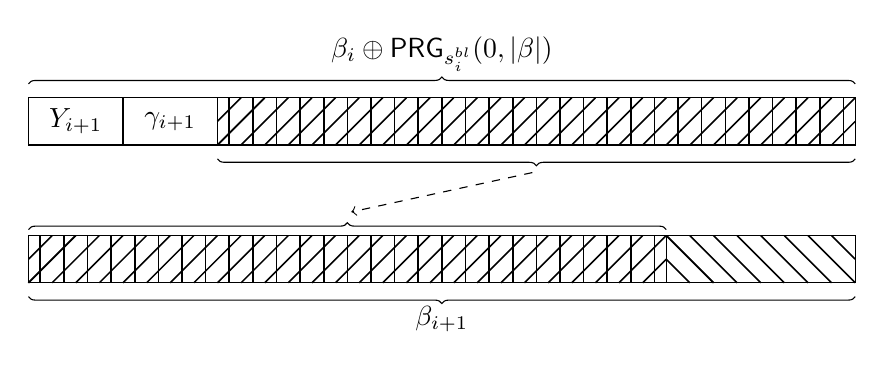
\begin{tikzpicture}
        \def\betaLength{10.5}
        \def\pubKey{1.2}
        \def\authTag{1.2}
        \def\one{0.6}
        \draw (0,0) rectangle (\betaLength,\one);

        \draw (0,0) rectangle (\pubKey,\one) node[midway] {$Y_{i+1}$};
        \draw (\pubKey,0) rectangle (\pubKey+\authTag,\one) node[midway] {$\gamma_{i+1}$};

        \draw[decoration={brace,raise=5pt},decorate] (0,\one) -- (\betaLength,\one) node [midway,above=6pt] {$\beta_i \oplus \textsf{PRG}_{s_i^{bl}}(0, | \beta |)$};

        \draw[decoration={brace,raise=5pt,mirror},decorate] (\authTag+\pubKey,0) -- (\betaLength,0);

        \def\halfBeta{{(\betaLength-\pubKey-\authTag)}*0.5}
        \draw [->,dashed] (4.0+\pubKey+\authTag, -0.35) -- (4.1, -0.85);

        \draw[decoration={brace,raise=5pt},decorate] (0,-1.25) -- (\betaLength-\authTag-\pubKey,-1.25);

        \begin{scope}[shift={(\pubKey+\authTag,0)}]
            \def\a{8.1}
            \def\b{\one}
            \def\lw{0.2}
            \def\diff{7.5}

            \foreach \x [count=\i] in{0,0.3,0.6,...,\b}{
                    \draw [line width=\lw mm](0,\x)--(\b-\x,\b) (\a-\b+\x,0)--(\a,\b-\x);
                }
            \foreach \x [count=\i] in{0,0.3,0.6,...,\diff}{
                    \draw [line width=\lw mm](\x,0)--(\b+\x,\b);
                }

            \foreach \x [count=\i] in{0,0.15,0.45,...,\a}{
                    \draw [line width=\lw mm](\x,0)--(\x,\b);
                }
        \end{scope}

        \begin{scope}[shift={(0, -1.75)}]
            \draw (0,0) rectangle (\betaLength,\one);
            \draw[decoration={brace,raise=5pt,mirror},decorate] (0,0) -- (\betaLength,0) node[midway,below=5pt] {$\beta_{i+1}$};

            \draw (\betaLength-\pubKey-\authTag, 0) -- (\betaLength-\pubKey-\authTag,\one);

            \begin{scope}[shift={(0,0)}]
                \def\a{8.1}
                \def\b{\one}
                \def\lw{0.2}
                \def\diff{7.5}

                \foreach \x [count=\i] in{0,0.3,0.6,...,\b}{
                        \draw [line width=\lw mm](0,\x)--(\b-\x,\b) (\a-\b+\x,0)--(\a,\b-\x);
                    }
                \foreach \x [count=\i] in{0,0.3,0.6,...,\diff}{
                        \draw [line width=\lw mm](\x,0)--(\b+\x,\b);
                    }

                \foreach \x [count=\i] in{0,0.15,0.45,...,\a}{
                        \draw [line width=\lw mm](\x,0)--(\x,\b);
                    }
            \end{scope}

            \begin{scope}[shift={(\betaLength-\pubKey-\authTag,0)}]
                \def\a{2.4}
                \def\b{0.6}
                \def\lw{0.2}
                \def\diff{1.8}
                \foreach \x [count=\i] in{0,0.3,0.6,...,\b}{
                        \draw [line width=\lw mm](\x,0)--(0,\x) (\a-\b+\x,\b)--(\a,\x);
                    }
                \foreach \x [count=\i] in{0,0.3,0.6,...,\diff}{
                        \draw [line width=\lw mm](\x+\b,0)--(\x,\b);
                    }
            \end{scope}
        \end{scope}

    \end{tikzpicture}
    \caption{Shifting in the header}
\end{figure}